\chapter{Ejercicio 3}


\section{Consigna}

En este ejercicio se implementará una maquina de estados de Moore siguiendo lo solicitado por el trabajo y luego se hará una máquina de estados equivalente en su versión Mealy. Esta máquina es la que se muestra a continuación:\\

\begin{figure}[H]
\begin{center}
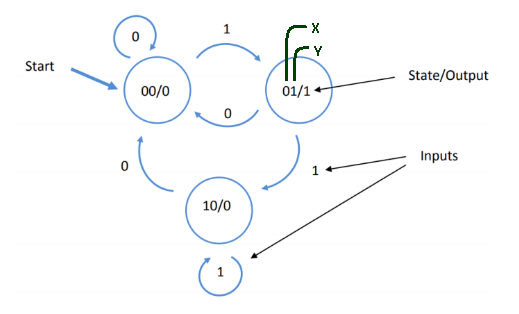
\includegraphics[scale=0.8]{../Ejercicio-3/imagenes/consigna.png}
\end{center}
\caption{Maquina de estados solicitada}

\end{figure}


\section{Maquina de estado de Moore}

Como se sabe las maquinas de estado de Moore se caracterizan por tener una salida unicamente dependiente del estado actual del sistema, sin depender de forma instantánea de la entrada.\\

Como primera instancia para resolución de esta máquina se define que valores para los bits denominados como \emph{X} e \emph{Y }, ilustrados en la figura anterior, caracterizan a cada uno de los estados, se puede observar ademas que cuando ambos de estos bits valen 1 la maquina no se encuentra en ningún estado relevante por lo que este se tratara como un estado de \emph{don\textasciiacute t care}. En la siguiente tabla se resume todo esto:\\

\begin{figure}[H]
\begin{centering}
\begin{tabular}{|c|c|c|}
\hline 
\multirow{2}{*}{Estados} & \multicolumn{2}{c|}{Condiciones}\tabularnewline
\cline{2-3} 
 & \multicolumn{1}{c|}{X} & Y\tabularnewline
\hline 
A & 0 & 0\tabularnewline
\hline 
B & 0 & 1\tabularnewline
\hline 
C & 1 & 0\tabularnewline
\hline 
\emph{don\textasciiacute t care} & 1 & 1\tabularnewline
\hline 
\end{tabular}
\par\end{centering}
\caption{Condiciones de estados}

\end{figure}

Una vez definido que valores identifican a cada uno de los estados lo que sigue es recopilar la información sobre como evoluciona el sistema según las entradas a este y como también cada estado determina la salida obtenida del sistema, todo esto se resume en la siguiente tabla:\\

\begin{figure}[H]
\begin{centering}
\begin{tabular}{|c|c|c|c|c|c|c|}
\hline 
\multicolumn{2}{|c|}{Estado Actual} & \multicolumn{4}{c|}{Estado futuro} & \multirow{3}{*}{Output}\tabularnewline
\cline{1-6} 
\multirow{2}{*}{x} & \multirow{2}{*}{y} & \multicolumn{2}{c|}{input = 0} & \multicolumn{2}{c|}{input = 1} & \tabularnewline
\cline{3-6} 
 &  & X & Y & X & Y & \tabularnewline
\hline 
0 & 0 & 0 & 0 & 0 & 1 & 0\tabularnewline
\hline 
0 & 1 & 0 & 0 & 1 & 0 & 1\tabularnewline
\hline 
1 & 0 & 0 & 0 & 1 & 0 & 0\tabularnewline
\hline 
1 & 1 & \emph{d} & \emph{d} & \emph{d} & \emph{d} & \emph{d}\tabularnewline
\hline 
\end{tabular}
\par\end{centering}
\caption{State assigned table}

\end{figure}

Nótese que se utilizaran letras minúsculas para designar estados actuales y letras mayúsculas para estados futuros.\\

Tanto la información sobre los estados futuros como de la salida se pueden contener en una tabla de verdad teniendo como variables los estados actuales \emph{x} e \emph{y} y el valor de entrada:\\

\begin{figure}[H]
\begin{centering}
\begin{tabular}{|c|c|c||c|c|}
\hline 
input & x & y & X & Y\tabularnewline
\hline 
\hline 
0 & 0 & 0 & 0 & 0\tabularnewline
\hline 
0 & 0 & 1 & 0 & 0\tabularnewline
\hline 
0 & 1 & 0 & 0 & 0\tabularnewline
\hline 
0 & 1 & 1 & 0 & 0\tabularnewline
\hline 
1 & 0 & 0 & 0 & 1\tabularnewline
\hline 
1 & 0 & 1 & 1 & 0\tabularnewline
\hline 
1 & 1 & 0 & 1 & 0\tabularnewline
\hline 
1 & 1 & 1 & \emph{d} & \emph{d}\tabularnewline
\hline 
\end{tabular}\ %
\begin{tabular}{|c|c||c|}
\hline 
x & y & Output\tabularnewline
\hline 
\hline 
0 & 0 & 0\tabularnewline
\hline 
0 & 1 & 1\tabularnewline
\hline 
1 & 0 & 0\tabularnewline
\hline 
1 & 1 & \emph{d}\tabularnewline
\hline 
\end{tabular}
\par\end{centering}
\caption{Tablas de verdad}

\end{figure}

Como se puede ver queda implícito en la tabla anterior que esta será una maquina de estado de Moore ya que la salida esta unicamente determinada por el estado actual.\\

Teniendo ya estas tablas de verdad se procede a utilizar el método de resolución con min-terminos del mapa de Karnaugh para obtener las expresiones lógicas de \emph{X} e \emph{Y} y de la salida, se
utilizarán los estados de \emph{don\textasciiacute t care} para lograr una expresión lo mas compacta posible, se aclara que \emph{y1} y \emph{y2} representan a \emph{x} e \emph{y} respectivamente mientras que W denota el valor de entrada:\\

\begin{figure}[H]
	\centering
	\begin{Karnaughvi}
		\contingut{0,0,0,X,0,1,1,X}
		\implicant{5}{7}{red}
		\implicant{7}{6}{green}
	\end{Karnaughvi}
\caption{Mapa de Karnaugh de X}
\end{figure}

\begin{figure}[H]
\centering
	\begin{Karnaughvi}
		\contingut{0,0,0,X,1,0,0,X}
		\implicant{4}{4}{red}
	\end{Karnaughvi}
\caption{Mapa de Karnaugh de Y}
\end{figure}

\begin{figure}[H]
\centering
	\begin{Karnaughquatre}
		\contingut{0,0,1,X}
		\implicant{2}{3}{red}
	\end{Karnaughquatre}

\caption{Mapa de Karnaugh de Output}
\end{figure}

Las expresiones obtenidas son las siguientes:\\
\begin{itemize}
\item $X=inp\cdot x+inp\cdot y=inp\cdot(x+y)$
\item $Y=inp\cdot\overline{x}\cdot\overline{y}$
\item $Output=y$
\end{itemize}
Las cuales describen el comportamiento del siguiente circuito:\\

\begin{figure}[H]
\begin{centering}
\includegraphics[scale=0.8]{../Ejercicio-3/\string"imagenes/E3 TP3 Moore\string".png}
\par\end{centering}
\caption{Circuito de Moore}
\end{figure}


\section{Maquina de estado de Mealy}

Mientras que la maquina de estados de Moore depende exclusivamente del estado actual del sistema la de Mealy no solo depende de este sino también del que se tiene a la entrada del sistema, de allí una de las principales diferencias con respecto a las maquinas de estado de Moore, un cambio a la entrada se verá reflejado \emph{instantáneamente} a la salida.\\

Para llegar a que la salida esté en relación directa con la entrada se analizó paso a paso el comportamiento del sistema. Se entiende que la maquina verá un 1 a su salida cuando se tenga un 1 a la entrada y simultaneamente se esté en un estado latente o inicial, una vez muestreado este valor se pasará a un nuevo estado en el cual el sistema arrojará 0 ante cualquier salida. En este estado se permanecerá mientras se siga leyendo un 1 a la entrada y se regresará al estado inicial en
caso contrario. A continuación un ejemplo:\\

\begin{figure}[H]
\begin{centering}
\begin{tabular}{|c|c|c|c|c|c|c|c|c|}
\hline 
 & $t_{0}$ & $t_{1}$ & $t_{2}$ & $t_{3}$ & $t_{4}$ & $t_{5}$ & $t_{6}$ & $t_{7}$\tabularnewline
\hline 
\hline 
Input & 0 & 1 & 0 & 1 & 1 & 1 & 0 & 1\tabularnewline
\hline 
Output & 0 & 1 & 0 & 1 & 0 & 0 & 0 & 1\tabularnewline
\hline 
\end{tabular}
\par\end{centering}
\caption{Ejemplo de funcionamiento de la maquina}

\end{figure}

Visto el comportamiento de la máquina se propone el siguiente esquema para este:\\

\begin{figure}[H]
\begin{centering}
\includegraphics[scale=0.8]{../Ejercicio-3/\string"imagenes/E3 TP3 Mealy paint\string".png}
\par\end{centering}
\caption{Esquema de la maquina de Mealy}

\end{figure}

Del mismo modo que antes se puede representar el funcionamiento de la maquina en la siguiente tabla:\\

\begin{figure}[H]
\begin{centering}
\begin{tabular}{|c|c|c|c|c|}
\hline 
\multirow{2}{*}{Estado actual} & \multicolumn{2}{c|}{Estado futuro} & \multicolumn{2}{c|}{Output}\tabularnewline
\cline{2-5} 
 & input = 0 & input = 1 & input = 0 & input = 1\tabularnewline
\hline 
A & A & B & 0 & 1\tabularnewline
\hline 
B & A & B & 0 & 0\tabularnewline
\hline 
\end{tabular}
\par\end{centering}
\caption{State assigned table}

\end{figure}

Como se ha planteado hasta ahora solo existen 2 estados posibles por lo tanto si se considera la variable \emph{estados} (la cual se llamara \emph{x} para los presentes y \emph{X} para los futuros) se puede
decir que esta nueva variable posee un valor binario, 0 para el estado A y 1 para el estado B. Desde aquí se puede implementar la siguiente tabla de verdad:\\

\begin{figure}[H]
\begin{centering}
\begin{tabular}{|c|c||c|c|}
\hline 
x & input & X & Output\tabularnewline
\hline 
\hline 
0 & 0 & 0 & 0\tabularnewline
\hline 
0 & 1 & 1 & 1\tabularnewline
\hline 
1 & 0 & 0 & 0\tabularnewline
\hline 
1 & 1 & 1 & 0\tabularnewline
\hline 
\end{tabular}
\par\end{centering}
\caption{Tablas de verdad}

\end{figure}

Desde aquí es fácil observar las siguientes implicaciones lógicas:\\
\begin{itemize}
\item $X=inp$
\item $Output=inp\cdot\overline{x}$
\end{itemize}
Las cuales se representan el funcionamiento del siguiente circuito:\\

\begin{figure}[H]
\begin{centering}
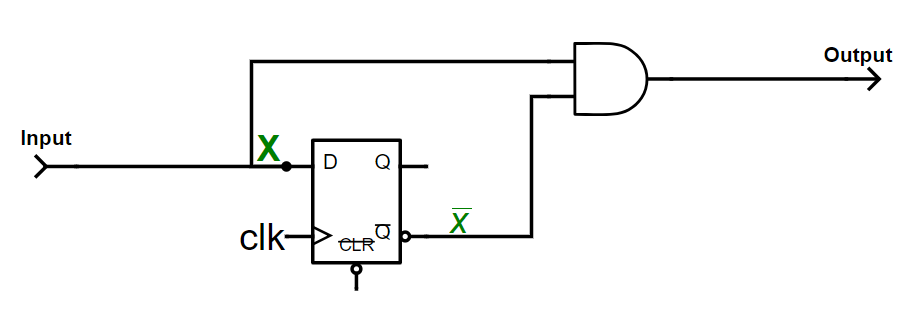
\includegraphics[scale=0.8]{../Ejercicio-3/imagenes/E3-TP3-Mealy.png}
\par\end{centering}
\caption{Circuito de Mealy}

\end{figure}

\section{Conversión de tensiones}

Una condición para el diseño de los circuitos es que estos reciban y devuelvan tensiones de 0 o 5V mientras que la lógica interna de esta debe operar a 3.3V, por lo que se deberá implementar tecnología que trabaje con este nivel de tensión realizando la respectiva conversión de voltaje tanto a la entrada como a la salida.\\

Para esto último se utilizó el circuito integrado SN7407N el cual permite realizar cómodamente una conmutación de tensión dado que se le permite al usuario operar con el colector del transistor ubicado a la salida de este, es decir, este es un dispositivo \emph{open-colector}. Un diagrama simplificado de su funcionamiento se muestra a continuación:\\

\begin{figure}[H]
\begin{centering}
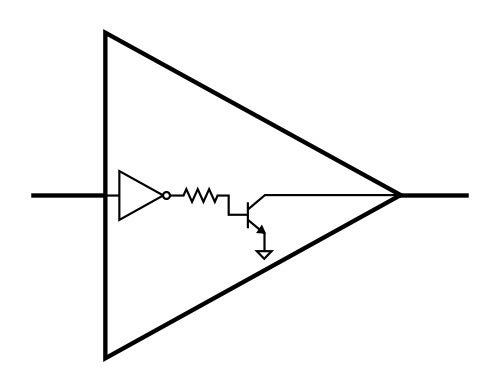
\includegraphics[scale=1.2]{../Ejercicio-3/imagenes/SN7407N.jpg}
\par\end{centering}
\caption{Diagrama del SN7407N}

\end{figure}

Como se puede ver un 1 lógico a la entrada dejara en alta impedancia la salida del integrado, dado que el transistor estará en estado de corte, con lo cual implementado una resistencia de pull-up sobre el colector a la salida se tendrá la tensión deseada.\\

\section{Resultados obtenidos}
Ya con los esquematicos y la estructura del circuito definida se procedio a realizar la implementación de esta. Finalmente el circuito se comportó conforme a lo esperado lo cual se muestra en las siguientes imagenes que se consideraron suficientemente representativas:\\

\begin{figure}[H]
\begin{centering}
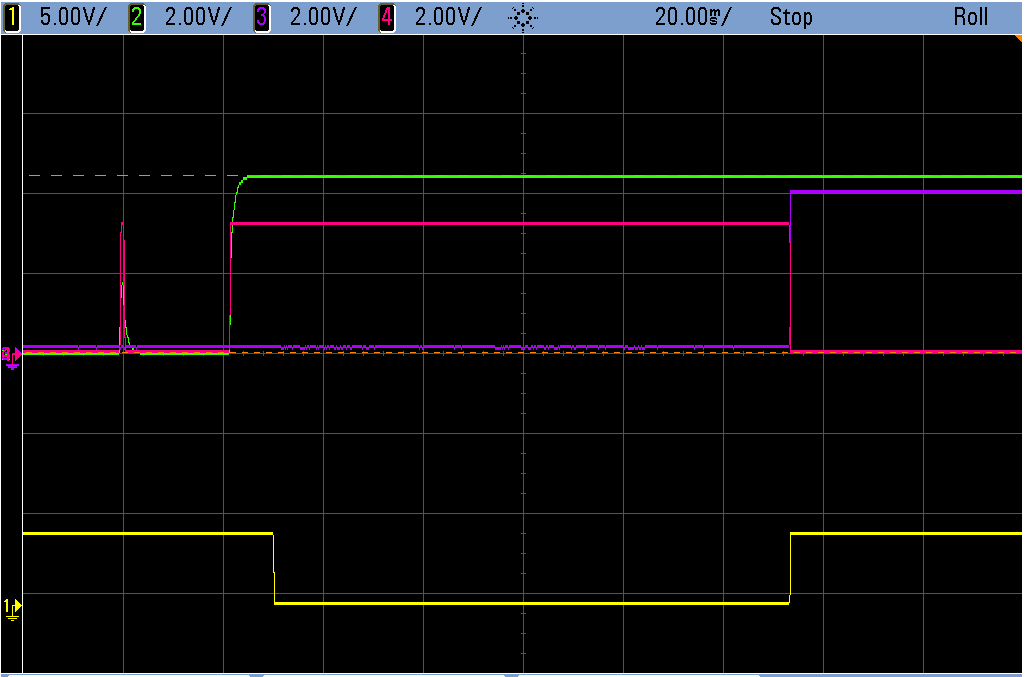
\includegraphics[scale=0.5]{../Ejercicio-3/imagenes/e3_tp3.png}
\par\end{centering}
\caption{Transisión de estados}

\end{figure}

\begin{figure}[H]
\begin{centering}
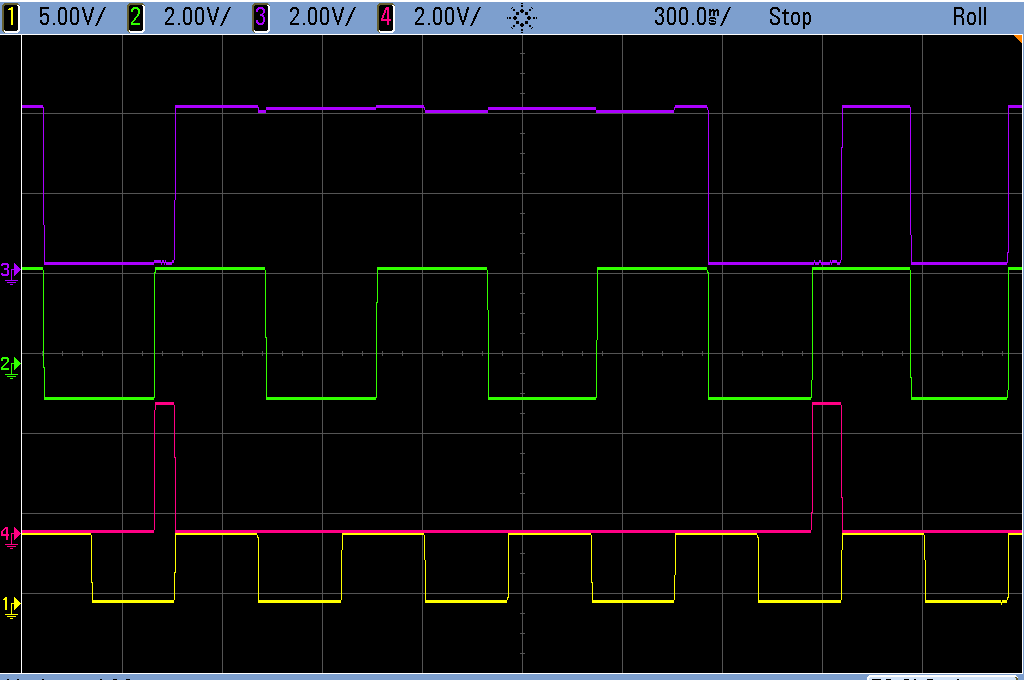
\includegraphics[scale=0.5]{../Ejercicio-3/imagenes/e3_tp3_b.png}
\par\end{centering}
\caption{Transisión de estados}

\end{figure}

En las figuras anteriores, las cuales pertenecen al circuito de Mealy, se tiene el clock como la señal amarilla, la señal de input como verde, la salida no negada del flip-flop como la violeta y finalmente la salida del circuito como rosada. Se observa al comnutar la entrada al valor HIGH en el intervalo de tiempo compendido este evento y el flanco positivo del clock se tiene que la salida del será también HIGH, regresando al valor LOW cuando se alcanza dicho el flanco positivo.
